\documentclass[a4paper,12pt]{article}
\usepackage[utf8]{inputenc}
\usepackage[T1]{fontenc}
\usepackage[ngerman]{babel}
\usepackage {amsmath}
\usepackage{amsfonts}
\usepackage{graphicx}

\title{Erklärung}

\begin{document}

\section{Erklärung}
\subsection{Das Shortest-Path Problem}
Das Shortest-Path Problem ist in der Literatur manchmal auch unter dem Namen Single-Source Shortest Path Problem zu finden. 
Es behandelt die Frage, wie man in einem Graphen ausgehend von einem gegebenen Anfangsknoten s (engl. Source) zu jedem anderen Knoten des Graphen den kürzesten Pfad findet \footnote{OTTMANN, Thomas; WIDMAYER Peter: Algorithmen und Datenstrukturen, Reihe Informatik Bd. 70, Mannheim: BI-Wissenschaftsverlag, 1990, S. 572, Z. 19-20}. Mit kurz ist hierbei nicht die Länge gemeint, sondern die Minimierung der Kantenkosten. Im Allgemeinen ist mit Länge nicht die tatsächliche Länge gemeint, sondern die Pfadkosten.

\subsection{Mathematische Definition}

[HIER DEFINITION EINFÜGEN, AD Skript S.132]

\subsection{Zur Eingabe}
Die Eingabe besteht stets aus gerichteten Graphen. Hierbei muss jedoch angemerkt werden, dass sich jeder ungerichtete Graph leicht in einen gerichteten Graph umwandeln lässt, indem man für jede Kante \{u,v\} die Kanten (u,v) und (v,u) mit gleichen Kosten einführt.\footnote{AD Skript, S.133 Z.8-13} Somit findet der Dijkstra-Algorithmus auch für ungerichtete Graphen Anwendung, solange man sie vorher in einen Digraphen überführt. 

\parindent0pt Zudem wird davon ausgegangen, dass die Kantenkosten nicht negativ sind.

\subsection{Das Optimalitätsprinzip}
Dem Dijkstra-Algorithmus liegt das Optimalitätsprinzip zugrunde:

\parindent0pt Für jeden kürzesten Pfad p=(v{\tiny 0},v{\tiny 1},...,v{\tiny k}) von v{\tiny 0} nach v{\tiny k} ist jeder Teilweg p'=(v{\tiny i}, ..., v{\tiny j}) mit $0 \le i < j \le k$ ein kürzester Weg von v{\tiny i} nach v{\tiny j}.

\parindent0pt Das bedeutet kurz gesagt, dass man für alle möglichen Teilpfade annimmt, dass sie optimal sind.
Dass diese Annahme stimmt, lässt sich mittels Widerspruchbeweis nachweisen: 

\parindent0pt Man geht vom Gegenteil aus, nämlich dem Fall, dass neben dem Pfad p' von v{\tiny i} nach v{\tiny j} ein anderer, kürzerer Pfad p'' von v{\tiny i }nach v{\tiny j} existiert. Dann müsste man p' durch p'' ersetzen (denn p'' ist kürzer). Damit würde sich auch der Gesamtpfad von v{\tiny 0} nach v{\tiny k} verkürzen. Da unser Pfad p von v{\tiny 0} nach v{\tiny k} bereits der kürzeste war, ist das  ein Widerspruch. \footnote{OTTMANN, Thomas; WIDMAYER Peter: Algorithmen und Datenstrukturen, Reihe Informatik Bd. 70, Mannheim: BI-Wissenschaftsverlag, 1990, S.573, Z.1-5}


\subsection{Funktionsweise des Algorithmus}
Auf welche Weise findet man nun zur optimalen Lösung?
Die Grundidee besteht darin, für jeden Knoten die Pfadkosten zu schätzen und die bestehende Lösungsmenge mit dem Knoten zu erweitern, welcher den geringsten Schätzwert aufweist. 

\parindent0pt Diese Arbeitsweise entspricht dem Greedy-Entwurfsmuster (engl. gierig): Nach einem Auswahlkriterium (die sogenannte Greedy-Regel) wird aus einer Menge das Element zur Erweiterung der Lösung gewählt, das den meisten Nutzen verspricht. In diesem Fall ist die Greedy-Regel das Verlangen nach dem kleinsten Schätzwert.

\parindent0pt Dijkstra geht bei seinem Algorithmus folgendermaßen vor: Er unterteilt die Knoten des Graphen zunächst einmal in drei Gruppen: Die Knoten, deren Schätzwert bereits feststehen ("black nodes"\footnote{DIJKSTRA Edsger W., FEIJEN W.H.J.: A Method of Programming,Cornwall: Addison-Wesley Publishing Company,1988, S.107 Z.24}), deren Nachfolger ("grey nodes"\footnote{vergl. Ebd., S.108, Z.2-3} sowie unerreichbare Knoten, deren Schätzwerte gänzlich unbekannt sind ("white nodes" \footnote{vergl. Ebd., S.108, Z.3}).

\begin{figure}[h]
\centering
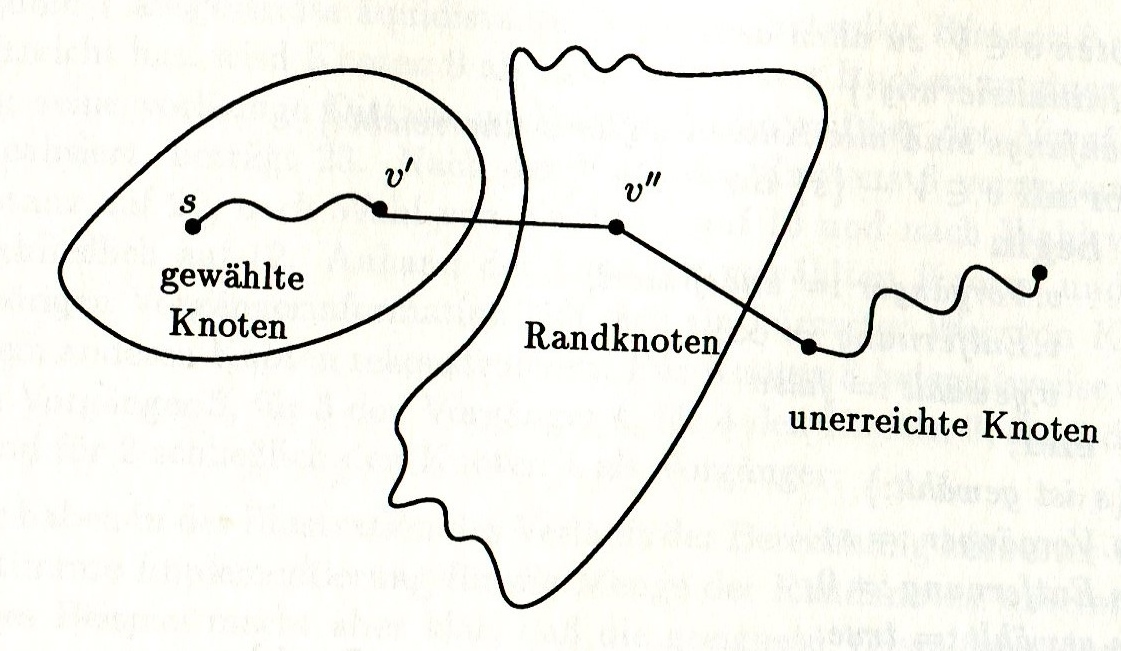
\includegraphics[width = 8cm]{knotentypen.jpg}
\caption{Knotentypen {\tiny (Quelle: OTTMANN, Thomas; WIDMAYER Peter: Algorithmen und Datenstrukturen, Reihe Informatik Bd. 70, Mannheim: BI-Wissenschaftsverlag, 1990, S.573 Abb. 8.19)} }
\label{a1}
\end{figure}


\parindent0pt Wenn keine grauen Knoten vorhanden sind, lässt sich die Lösungsmenge nicht erweitern. 

\parindent0pt Ansonsten muss aus den grauen Knoten einer ausgewählt werden, der schwarz werden soll, d.h. der Knoten, mit dem die Lösungsmenge erweitert wird. Alle vorherigen Pfade bestehen dabei ausschließlich aus schwarzen Knoten, d.h. Knoten die mit endgültig festgelegten Schätzwerten der Lösungsmenge bereits hinzugefügt wurden.

\parindent0pt Um zu bestimmen, welcher graue Knoten gewählt wird muss man die Kosten seines speziellen Pfades bestimmten \footnote{vergl. Ebd., S.108,Z.8-12}, d.h. den Pfad ausgehend vom Startknoten s bis hin zur Kante vom letzten schwarzen Knoten zum aktuellen grauen Knoten. Der Knoten, dessen spezieller Pfad am kostengünstigsten ist, wird in die Menge der schwarzen Knoten aufgenommen und aus der Menge der grauen entfernt. Ist dieser Schritt vollzogen, müssen noch seine Nachfolger behandelt werden. Dabei gibt es für jeden Nachfolger drei Möglichkeiten:

\parindent0pt Fall 1: Der Nachfolger ist weiß, d.h. er hat noch keinen Schätzwert. Dann wird dieser jetzt bestimmt und der Knoten wird grau.

\parindent0pt Fall 2: Der Nachfolger ist grau. Dann muss verglichen werden, ob der aktuelle Schätzwert geringer ist als der vorherige, und wenn dies zutrifft, wird der Wert entsprechend aktualisiert. (Das ist immer dann der Fall, wenn man einen kostengünstigeren Pfad für den entsprechenden Knoten gefunden hat.)

\parindent0pt Fall 3: Der Nachfolger ist schwarz. Dann steht sein Schätzwert bereits fest und er kann ignoriert werden.

\subsection{Realisierung}
Um dies umzusetzen, geht Dijkstra folgendermaßen vor: In einem Array werden die Farben der Knoten gespeichert. Ein weiteres Array dient der Speicherung der Schätzwerte. 

\parindent0pt Da der Knoten mit minimalen Pfadkosten nur aus den grauen gewählt wird, ist es sinnvoll, ein Feld für diese anzulegen, wobei eine Variable, die zugleich als Zeiger dient, deren Anzahl speichert.

\parindent0pt Des weiteren werden zu jedem Knoten deren unmittelbare Vorgänger gespeichert, sodass sich der vollständige Pfad zu jedem Knoten zurückverfolgen lässt (Rekursion).

\parindent0pt Eingegeben wird ein Graph zusammen mit Startknoten s und Zielknoten v. Ist v nicht von s aus erreichbar, sind die zurückgegeben Pfadkosten 0. Ansonsten wird die Länge zurückgegeben.

\parindent0pt Das konkrete Vorgehen sieht nun folgendermaßen aus: \\

\parindent0pt \underline{1. Initialisierung:} Alle Knoten werden auf weiß gesetzt, der Startknoten s wird grau.

\parindent0pt \underline{2. Erweiterung:} Der Knoten mit minimalem Schätzwert wird aus der Menge der grauen Knoten ausgewählt und herausgenommen. Er wird auf schwarz gesetzt, sein Schätzwert ist nun endgültig.

\parindent0pt \underline{3. Aktualisierung: }Nun werden alle Nachfolger betrachtet. Deren Schätzwerte werden gegebenenfalls aktualisiert, wenn deren Pfadkosten nun geringer sind. \\ 

\parindent0pt Der Algorithmus terminiert, wenn alle grauen Knoten abgearbeitet sind bzw. wenn der letzte Knoten schwarz ist. \\

[Anmerkung: Die genaue Implementierung steht auf S.111. Hab sie bei images reingepackt, falls ihr euch die mal angucken wollt]


\end{document}
